

\chapter{Material and methods} \label{ch:theory}

Machine learning (ML), the cornerstone of today’s artificial intelligence (AI) revolution, brings new promises to clinical practice using medical images\cite{varoquaux2022machine}. Deep learning (DL) is a branch of machine learning architectures
that attempts to model high-level abstractions in data using
multiple processing layers \cite{han2018classification}.  Recently, DL models have been achieving remarkable results in skin cancer classification tasks \cite{yu2016automated,nie2022recent}. In particular, convolutional neural networks (CNNs) have become the standard approach to handling computer vision problems. Compared with the traditional machine learning algorithms, which require complex feature engineering, DL can automatically learn robust feature representation and adapt to different fields and applications more easily \cite{li2020cnn}. In this research, I used a DL algorithm in an attempt to develop an automated classification system using dermoscopic images of different established skin disorders.


\begin{figure}[!h]
\centering
	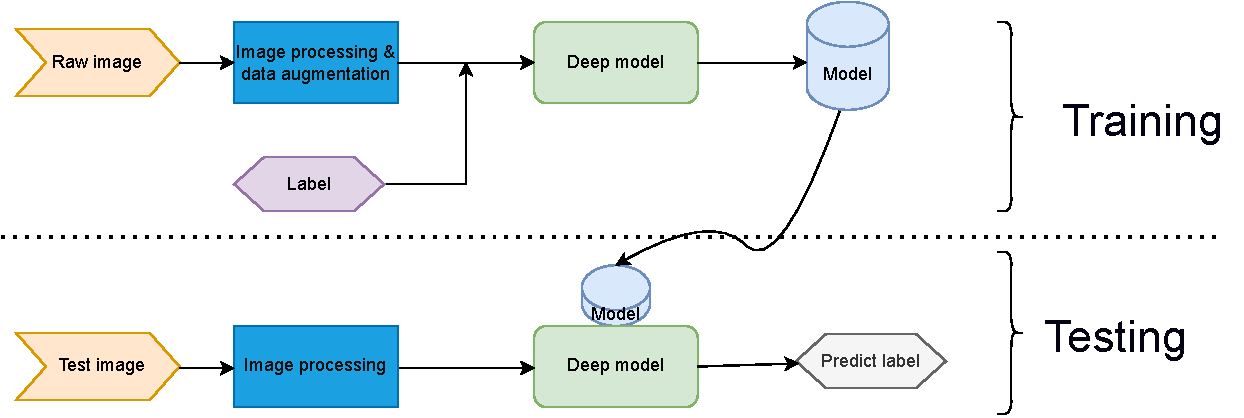
\includegraphics[width=4.2in]{CNN}
		\caption{Flow diagram of image classification based on deep learning.}
		\label{Fig:flow} 
\end{figure}

The whole process of image classification based on deep learning is illustrated in Figure \ref{Fig:flow}. The aim of image pre-processing is to improve the image data (i.e., features) by suppressing unwanted distortions and enhancing some important image features, so that the computer vision models can benefit from working on these improved data to work on. Model training is used to identify the most interesting patterns of the image, i.e., features that might be unique to a particular class and that will, later on, help the model to differentiate between different classes. 


\section{Image classification}

% \section{Methods} \label{section:stereo}

Image classification is the task of assigning a label or class to an entire image. Images are expected to belong to only one class each. Image classification models take an image as input and return a prediction about the class to which the image belongs.

 Classifying skin disease images with deep learning has the following steps:
\begin{itemize} \label{sec.step}
    \item Examine and understand data
    \item Build an input pipeline
    \item Build the model
    \item Train the model
    \item Test the model
    \item Improve the model and repeat the process
\end{itemize}
Choosing a good backbone model is an extremely important part of achieving good experimental results. In Figure \ref{Fig:model}, I give an example of the best backbone over the years.

The most highly used subset of ImageNet is the ImageNet Large Scale Visual Recognition Challenge (ILSVRC), 2012-2017, image classification and localization dataset. This dataset spans 1,000 object classes and contains 1,281,167 training images, 50,000 validation images, and 100,000 test images \cite{russakovsky2015imagenet}. ImageNet is a large labeled dataset of real-world images. It is one of the most widely used datasets in the latest computer vision research. A pre-trained image classification network that has already learned to extract powerful and informative features from natural images can be used as a starting point from which to learn a new task. Most of the pre-trained networks are trained on ImageNet.

\begin{figure}[!h]
\centering
	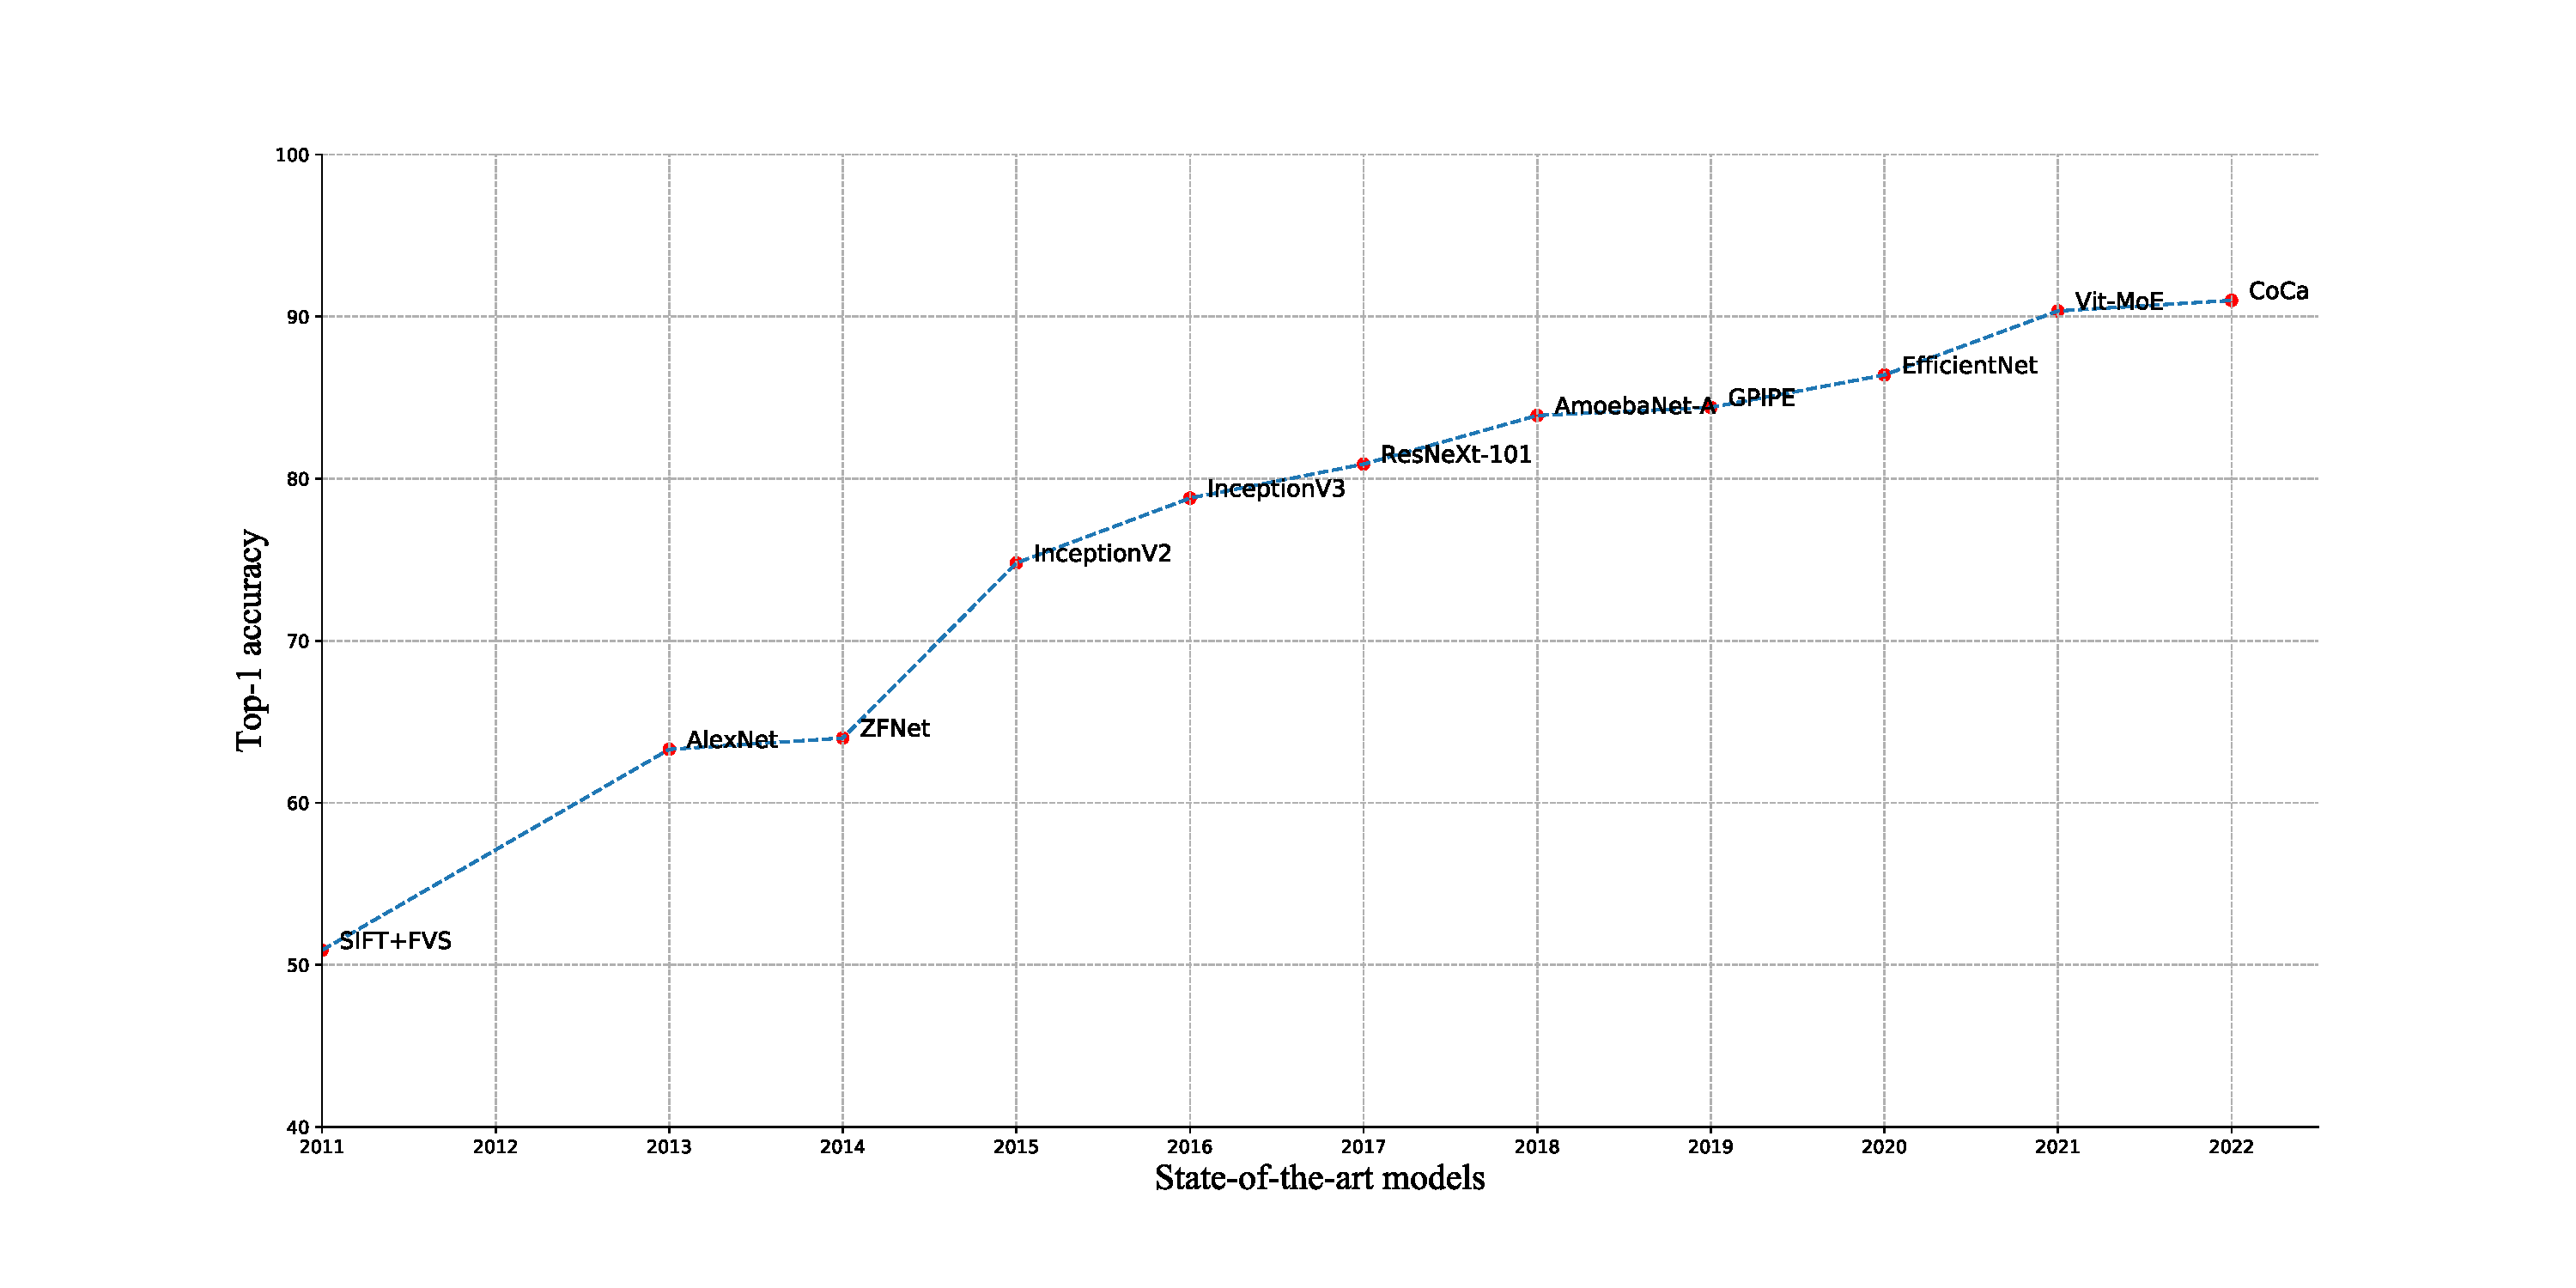
\includegraphics[width=5 in]{model_cla}
		\caption{Image classification: top-one accuracy on ImageNet from 2011 to 2022\cite{timmurphy.org}.}
		\label{Fig:model} 
\end{figure}


Figure \ref{Fig:model} shows the top-one accuracy for image classification on ImageNet from 2011 to 2022, extending from the dominance of CNN before 2021 to the emergence of ViT after 2021. Neural network backbones are also being constantly updated. CoCa \cite{yu2022coca} achieved SOTA 91.0$\%$ top-one accuracy on ImageNet with a finetuned encoder in 2022. It used attention pooling to fuse image-side information. As mentioned above, our papers \uppercase\expandafter{\romannumeral1}, \uppercase\expandafter{\romannumeral2}, \uppercase\expandafter{\romannumeral3}, \uppercase\expandafter{\romannumeral4}, and \uppercase\expandafter{\romannumeral6} all use these algorithms and techniques. Paper \uppercase\expandafter{\romannumeral5} is a review that mainly summarizes the use of CNNs in skin disease classification.

In paper \uppercase\expandafter{\romannumeral6}, I used a CNN-ViT hybrid model consisting of the following two modules: a CNN feature extractor and a transformer for spatial attention. First, the feature extractor module extracts the local visual features from input images. For feature extraction, I utilized a ResNet-50 network, which is a spatial transformer module consisting of six transformer encoders used to enhance spatial attention.

In papers \uppercase\expandafter{\romannumeral1} and \uppercase\expandafter{\romannumeral2}, I conducted a binary classification of skin lesions, i.e., benign or malignant, and used equal class data for training. In Paper \uppercase\expandafter{\romannumeral3}, I started using public datasets, which still contain binary classifications. However, in papers \uppercase\expandafter{\romannumeral4} and \uppercase\expandafter{\romannumeral6}, I used a slightly larger dataset with more than 10,000 images for experiments, and increased the number of categories to seven.

\section{Datasets}

Despite these technological advances, however, the lack of valid clinical datasets has limited the application of deep learning research in medicine. From Paper V, I summarize twelve fairly popular dermoscopic datasets, that are commonly used for skin cancer classification. The most famous one is the International Skin Imaging Collaboration (ISIC) dataset, used in an annual skin cancer classification competition since 2016. In Paper VI, I chose the ISIC-2018 dataset\cite{codella2019skin} as the experimental object and the lesion images come from the HAM10000 dataset \cite{tschandl2018ham10000}. In Paper IV, I used the HAM10000 dataset as training experiment data. These two databases are mutually inclusive and both have seven skin disease categories.

\begin{figure}[!h]
\centering
	\includegraphics[width=4.2in]{mel}
		\caption{Samples of each type of skin lesion from the ISIC 2018 dataset, where BCC and MEL are skin cancers (in the green dotted box), and others are common skin diseases\cite{codella2019skin}.}
		\label{Fig:mel} 
\end{figure}

In our work, I selected only 200 images from ISIC-2017\cite{codella2018skin}, half benign and half malignant, to ensure balanced categories in Paper I. In Paper II, the dataset was obtained from the University of Salerno, which collaborates with the University of Naples; this dataset has been accurately labeled by experts. Though there were only around 1,000 images, all of them have very high-quality annotations. I developed a CNN model-based 7-point skin lesion malignancy checklist, training, and testing it with the publicly available dataset Dermoscopy Atlas \cite{argenziano2000interactive} dataset, which contains 1011 dermoscopic images.


\begin{table}[!htbp]
\centering
\caption{The 7-point checklist criteria with related
individual scores.}\label{tab:point}
\begin{tabular}{p{9cm}c}
\toprule
\rowcolor{dGray}
\textbf{Clinical features}& \textbf{Score}\\
\midrule
\rowcolor{Gray}
\textit{Major criteria} &\\ 
%\rowcolor{gray!40}
\rowcolor{Gray}
Atypical pigment network & 2\\
\rowcolor{Gray}
Blue-whitish veil & 2\\
\rowcolor{Gray}
Atypical vascular pattern & 2\\
\midrule
\rowcolor{Lightgrey}
\textit{Minor criteria} & \\
\rowcolor{Lightgrey}
Irregular streaks & 1\\
\rowcolor{Lightgrey}
Irregular pigmentation& 1\\
\rowcolor{Lightgrey}
Irregular dots/globules & 1\\
\rowcolor{Lightgrey}
Regression structures& 1\\
\bottomrule
\end{tabular}
\begin{tablenotes}
        \footnotesize
        \item \textit{Note: A score of 3 or more is regarded as suspicious.}
      \end{tablenotes}
%\noindent{\footnotesize{A score of 3 or more is regarded as suspicious.}}
\end{table}


\begin{figure}[!h]
\centering
	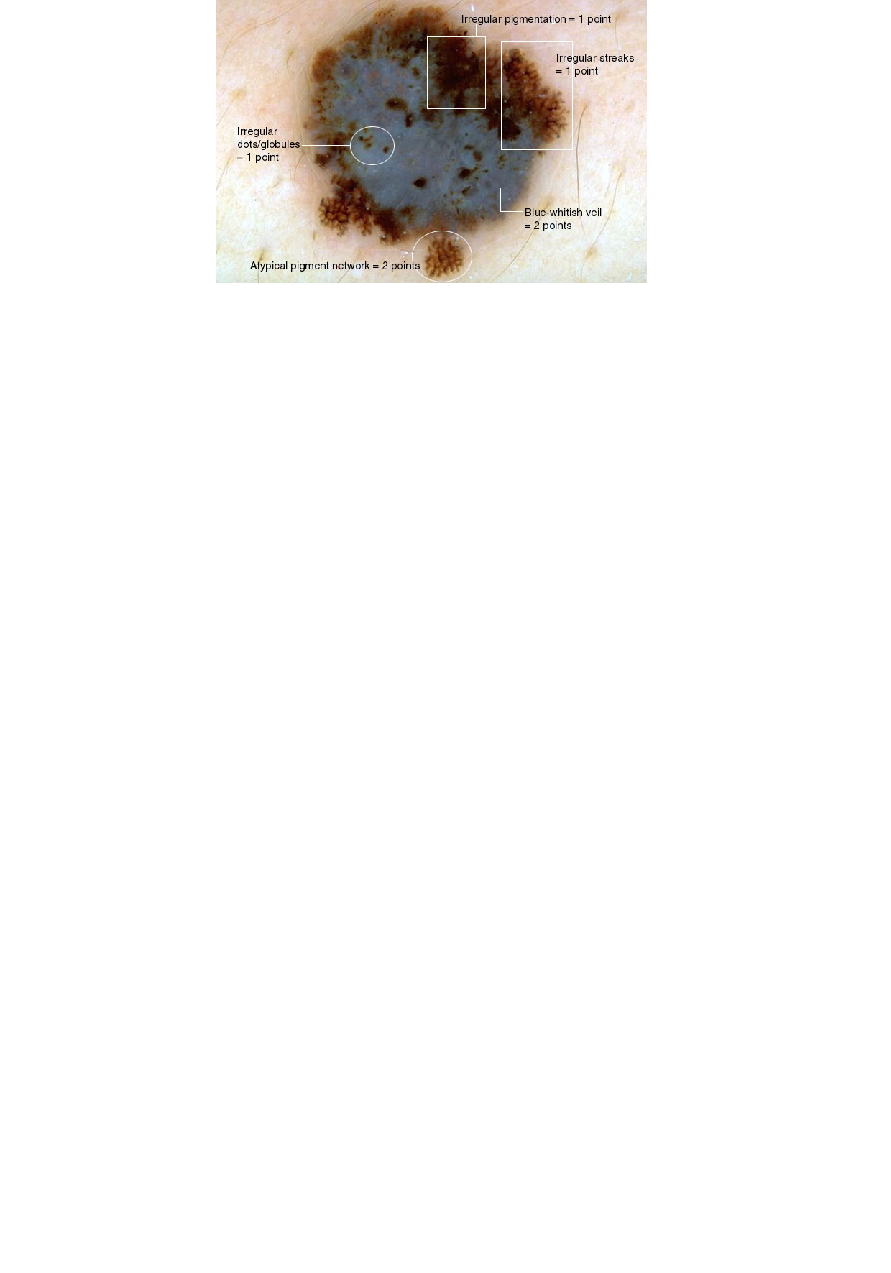
\includegraphics[width=4.2in]{7point}
		\caption{A diagnostic example of a 7-point checklist,  different structures are present and a score of seven is reached \cite{di2004elm}.}
		\label{Fig:7point} 
\end{figure}

The 7-point checklist is a diagnostic method that requires the identification of  seven dermoscopic criteria, i.e., features were selected for their frequent association with melanoma). These seven features refer both to the chromatic characteristics and to the shape and/or texture of the lesion. Dermoscopic images of a melanocytic skin lesion are analyzed for  evidence of the presence of these standard criteria; from this analysis, a score is calculated; finally, if a total score of three or more is attained, the lesion is classified as melanoma (otherwise it is classified as a benign). As for the individual criteria (see Table \ref{tab:point} and Figure \ref{Fig:7point}), there are three “major” criteria with individual scores of two and four “minor” criteria with individual scores of one.





\section{Image preprocessing}
"Garbage in, garbage out.” This slogan is common in computer science, mathematics in computer science, and machine learning. It refers to a very important point: even the best computer vision models will perform badly if the input data are of low quality. It is always crucial to strive to gather high-quality data for the current task. Additionally, even with high-quality data, preprocessing enables the best outcomes to be attained.

Image acquisition is the initial step in image classification. There are many potential sources of dataset bias in skin lesion imaging. Imaging devices or procedures may lead to specific measurement biases. A bias particularly harmful to clinically relevant automated diagnosis is when the data capture medical interventions. For instance, spurious correlations can appear in skin lesion images due to labeling errors.

Before being used for model training and inference, images usually first undergo image pre-processing. This includes, but is not limited to, resizing, orienting, and color corrections. The purpose of preprocessing is to increase the image's quality so that I can analyze it more effectively. Preprocessing allows us to eliminate unwanted distortions and improve specific qualities that are essential for the application I am working on. An image must be preprocessed for software to function correctly and produce the desired results.

There are several reasons for image preprocessing. First, CNNs' fully connected layers require that all the images be in arrays of the same size. Additionally, model preprocessing may shorten model training time and speed up model inference. If the input images are very large, shrinking their size  will greatly decrease the amount of time needed to train the model without significantly affecting model performance. 

\section{Data augmentation}
During the experiment, overfitting and underfitting are assessed in terms of the training error and test error. During the continuous iterative training process of the deep neural network model, the training error constantly decreases; however, after the test error drops to a certain point, it starts to rise. In Figure \ref{Fig:fit}, $t$ represents an inflection point. Before this inflection point has been reached, the neural network model has not reached the optimal state and the model can be considered underfitted. After the $t$ inflection point has been reached, although the training error continues to decrease, the test error starts increasing. This is because, although the training set fits very well, the model's generalization ability is poor and the test set does not perform well. Therefore, the model can be regarded as overfitted. In the case of poor model fitting, adding artificial data through data augmentation can effectively improve the effect of the network model.

\begin{figure}[!h]
\centering
	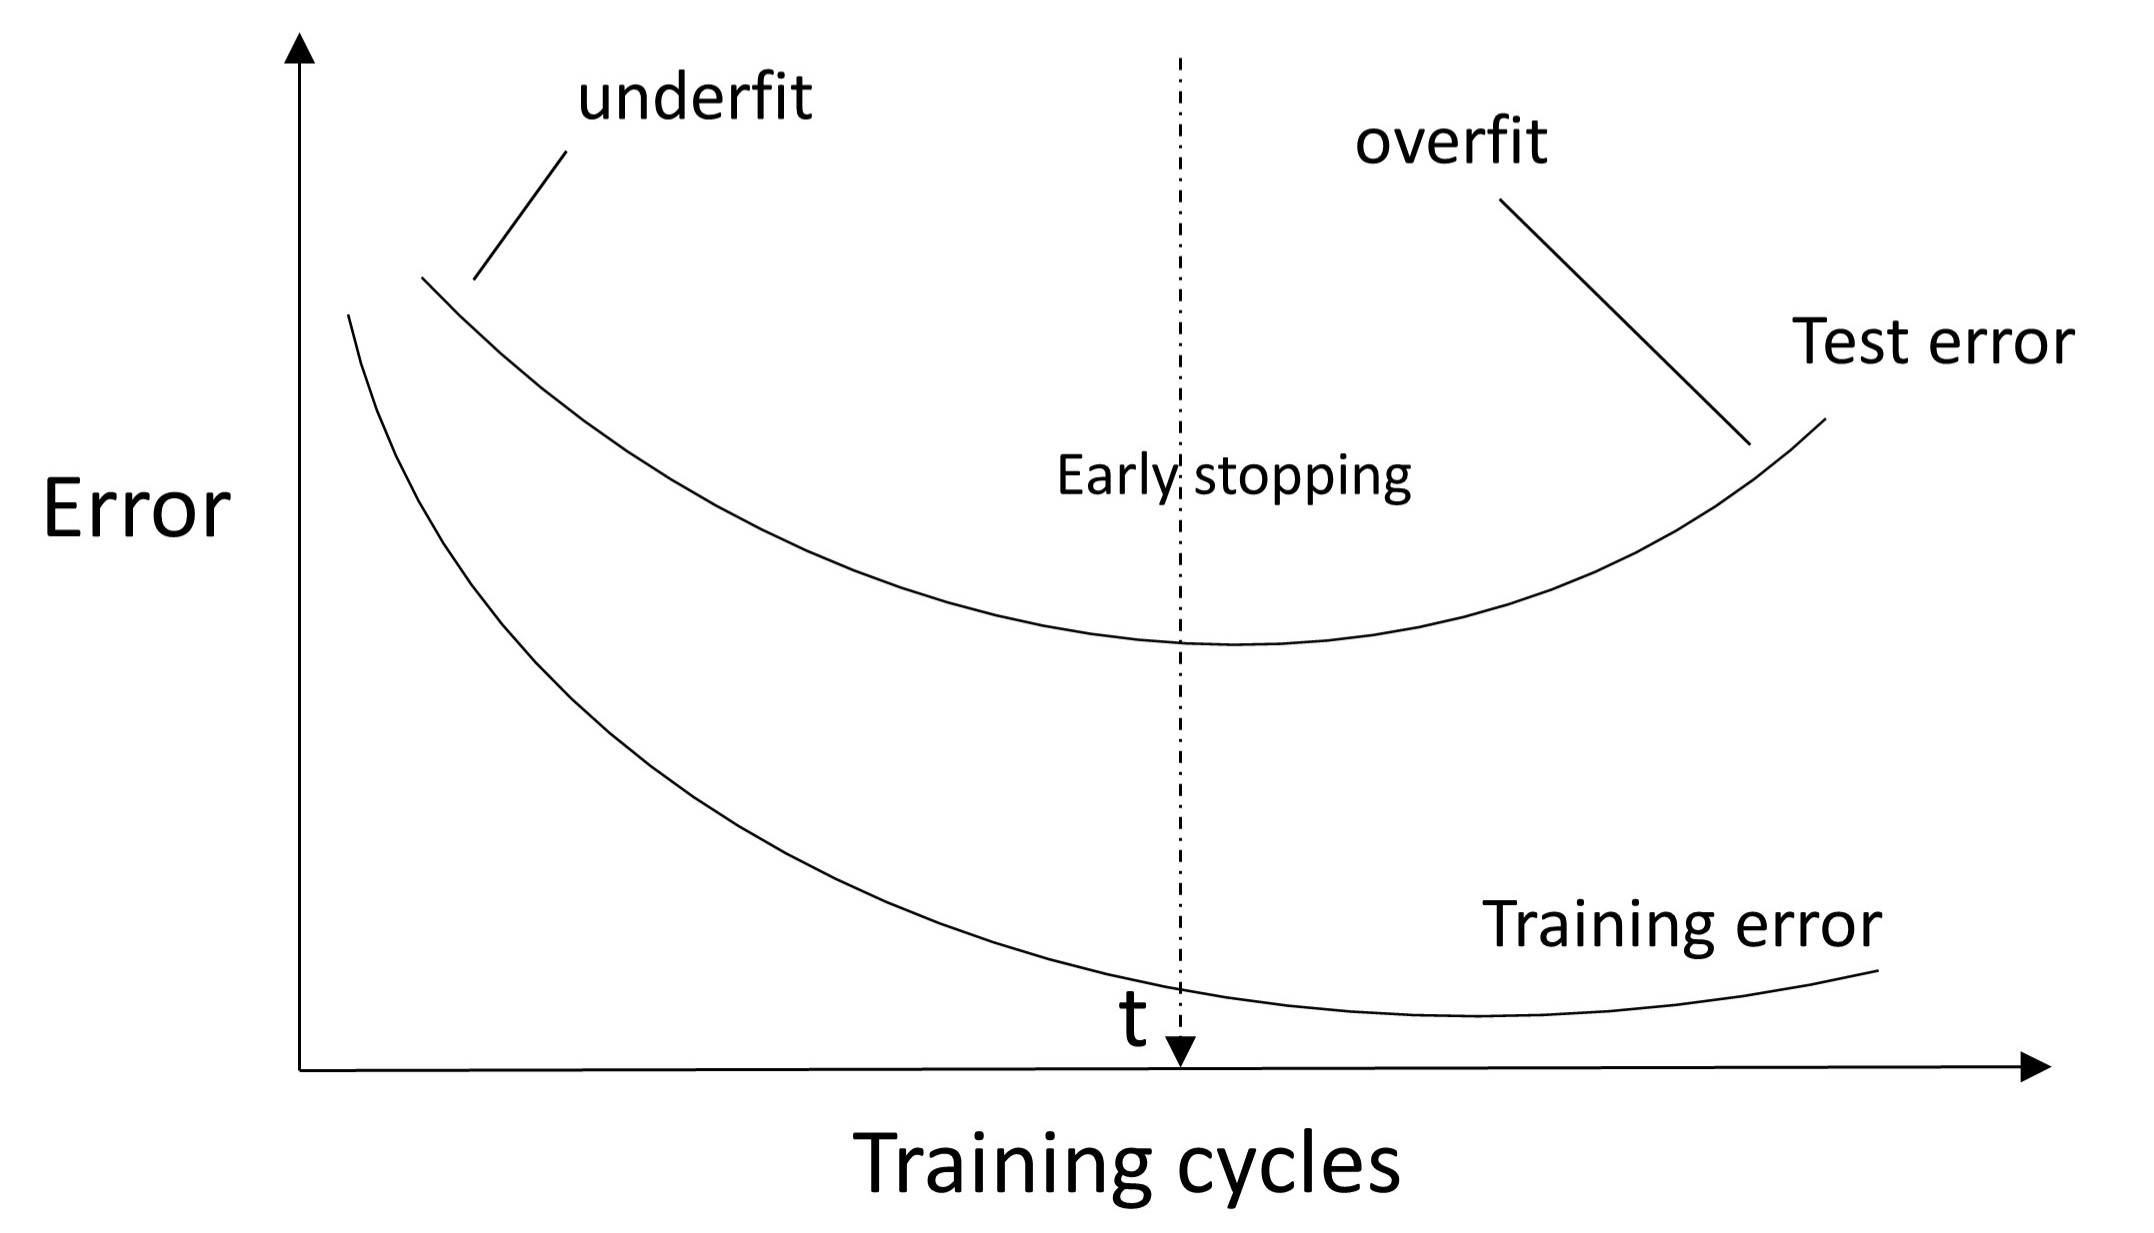
\includegraphics[width=3.2in]{overfit}
		\caption{Error during training and testing.}
		\label{Fig:fit} 
\end{figure}


Data augmentation is a manipulation applied to images to create different versions of similar content in order to expose the model to a wider range of training examples. For example, randomly altering the rotation, brightness, or scale of an input image requires that a model consider what an image subject looks like in a variety of situations.

Data augmentation manipulations are forms of image preprocessing, but there is a critical difference: while image preprocessing steps are applied to both training and test sets, image augmentation is only applied to the training dataset. Thus, a transformation that could be an augmentation manipulation in some situations may best be a preprocessing step in others.

\begin{figure}[!h]
\centering
	\includegraphics[width=4.2in]{aug}
		\caption{The difference between the original skin lesion image (left) and the images after data augmentation (right).}
		\label{Fig:aug} 
\end{figure}

It is impossible to truly capture an image that accounts for every real world scenario a model may encompass. This is where augmentation can help. By augmenting the images, I can increase the sample size of the training data and add new cases that might be hard to find in the real world. Augmenting existing training data to generalize to other situations allows the model to learn from a wider range of situations. This is particularly important when collected datasets may be small. A deep learning model will (over)fit to the examples shown in training, so creating variation in the input images enables the generation of new, useful training examples.


\section{Convolutional neural networks}  \label{sec:volumetric}
CNNs have the advantage of non-linear mapping by automatically adjusting the training weights between neurons. The standard CNN is basically composed of three layers: the convolutional, pooling, and fully connected layers. Figure \ref{Fig:vgg16} depicts the detailed structure of a Vgg-16 backbone network. The convolutional layer is the most important layer and performs most of the computation. It consists of kernels, which are composed of weights that learn visual features from the input images. Each kernel is convolved across the whole image and produces a feature map, which is the output of this layer. The pooling layer is basically used to reduce the feature map size. Consequently, it reduces the number of training parameters for the next layers, helps control overfitting, and, along with a non-linear activation filter, incorporates non-linearity into the network. The fully connected layer is a standard neural network that is connected to the last feature map provided by the previous layer. In summary, the composition of the convolutional and pooling layers is known as the feature extractor, and the fully-connected layer is the classifier.

\begin{figure}[!h]
\centering
	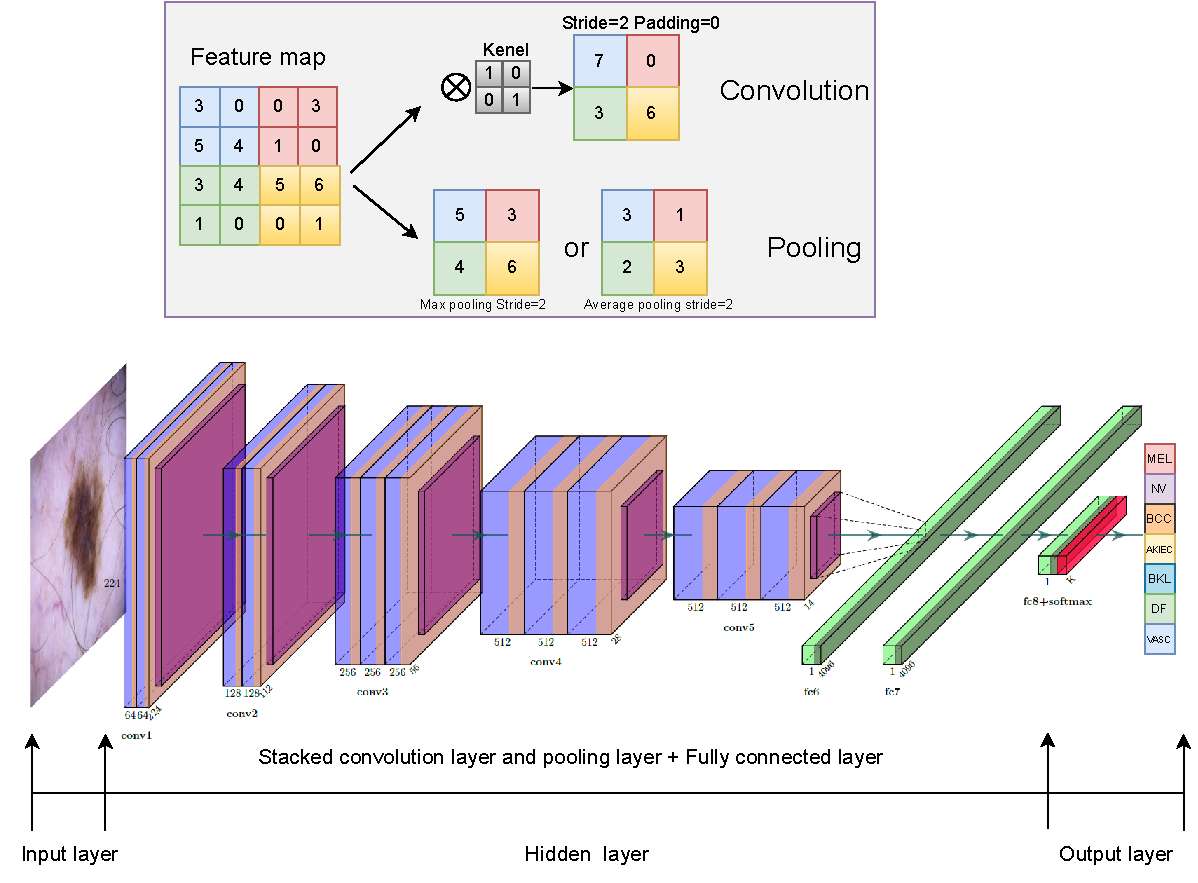
\includegraphics[width=4.2in]{VGG16_new}
		\caption{Illustration of the backbone network (Vgg-16) used to classify skin cancer images. First, the image features are extracted by the CNN feature extractor. Next, these features are reduced by the pooling layer. Finally, the softmax layer serves as the output layer of the model to predict skin lesion classes. \cite{haris_iqbal_2018_2526396,simonyan2014very}}.
		\label{Fig:vgg16} 
\end{figure}
%map of contributions to goals of research studies

CNNs have emerged as a powerful classification tool and are consistently used in object classification competitions, including the ImageNet challenge \cite{russakovsky2015imagenet}. Since AlexNet \cite{krizhevsky2017imagenet}, using CNN architecture, won the annual ILSVRC in 2012, CNN models such as Vgg\cite{simonyan2014very}, GoogLeNet\cite{szegedy2015going}, and ResNet\cite{he2016deep} have performed well in image recognition and classification. 

Different CNN architectures have been used to deal with skin cancer detection, and successful results have been reported by Steve et al. \cite{esteva2017dermatologist}. Nonetheless, for medical tasks, collecting a large number of data to train a CNN is challenging. To overcome this issue, most research has used transfer learning, a well-known technique in which a model trained for a given source task is partially reused for a new target task \cite{menegola2017knowledge}. In this way, models can be initialized using the weights from the ImageNet dataset \cite{russakovsky2015imagenet} and then fine-tuned using their own dataset. In our work, Paper \uppercase\expandafter{\romannumeral1} used Yolo1, Yolo2, and Yolo3; Paper \uppercase\expandafter{\romannumeral2} used Vgg-16; Paper \uppercase\expandafter{\romannumeral3} used GoogleNet, Inception-v3, and ResNet-101; Paper \uppercase\expandafter{\romannumeral4} used Vgg-19, ResNet-101 and Inception-V3; and Paper \uppercase\expandafter{\romannumeral6} used Resnet-50 as the baseline. These deep learning backbones are based on CNNs and are widely used in computer vision.

\section{Transformer neural networks}  \label{sec:trans}

A transformer model is a neural network that learns context and thus meaning by tracking relationships in sequential data such as the words in this sentence. The transformer neural network was first proposed by Vaswani et al. \cite{vaswani2017attention} in 2017 to solve some sequence-to-sequence tasks while handling long-range dependencies with a simple recurrent neural network (RNN). Vaswani et al. introduced an encoder-decoder architecture based on attention layers, which was called the transformer. Transformer models apply an evolving set of mathematical techniques, called attention or self-attention techniques, to detect subtle ways even distant data elements in a series influence and depend on one another.

Vision transformers (ViTs) use positional encoders to tag data elements coming in and out of the network. Attention units follow these tags, calculating a kind of algebraic map of how each element relates to the others. Attention queries are typically executed in parallel by calculating a matrix of equations in what is called multi-headed attention, as shown in detail in Figure \ref{Fig:trans}.

\begin{figure}[!h]
\centering
	\includegraphics[width=4.2in]{transformer}
		\caption{ViT model overview. The model splits an image into fixed-size patches, linearly embeds each of them, adds position embeddings, and feeds the resulting sequence of vectors into a standard transformer encoder. To perform classification, it uses the standard approach of adding an extra learnable “classification token * ” to the sequence \cite{dosovitskiy2020image}.}
		\label{Fig:trans} 
\end{figure}


Transformers are in many cases replacing convolutional and recurrent neural networks (CNNs and RNNs), the most popular types of deep learning models just five years ago \cite{whattran}. Before transformers arrived, users had to train neural networks with large labeled datasets that were costly and time-consuming to produce. By finding patterns between elements mathematically, transformers eliminate that need, making available the trillions of images and petabytes of text data on the web and in corporate databases. In addition, the math that transformers use lends itself to parallel processing, so these models can run quickly.

 A multi-head self-attention layer with a sufficient number of heads is at least as expressive as any convolutional layer \cite{cordonnier2019relationship}. However, pure transformer networks lack the inductive bias of CNNs and thus need to rely on large-scale data to achieve results comparable to those of CNNs. In Paper \uppercase\expandafter{\romannumeral6}, I used the hybrid Resnet-50 + Transformer model, which achieved good experimental results. In this paper, the input images were first passed through Resnet-50, and then the feature maps were sent to the transformer block. In this process, CNN can capture local features while Transformer will capture global features.

 




